\documentclass[hyperref={pdfpagelabels=false}]{beamer}
\setbeamercolor{background canvas}{bg=white}
\usepackage{graphicx,lmodern,subfigure,ulem,color,graphicx,tikz,booktabs,natbib}
\usepackage{subfig}
\usepackage{mathrsfs}
\usepackage{subfigure}
\usetheme{Warsaw}
%\definecolor{beamer@blendedblue}{rgb}{0.1,0.5,0.1}
%\definecolor{ForestGreen}{RGB}{60, 140, 60}
%\setbeamercolor{structure}{fg=beamer@blendedblue}
\setbeamertemplate{navigation symbols}{}
\setbeamertemplate{footline}[frame number]
\bibliographystyle{chicago}
\newcommand{\spitem}{\vspace{.3cm}\item}
\newcommand{\elas}{$E_{labor}$}
%\def \FigPath {Users\th3\Documents\Job_Market_Paper\Code\Figures} 
\DeclareMathOperator{\E}{\mathbb{E}}
\usepackage{makecell}




\title{ICT-Specific Investment Shocks and Economic Fluctuations}
%\\ \bigskip \\ \normalsize{Evidence and Theory of a General-Purpose Technology}
\author{Marco Brianti, Boston College\\Laura G\'ati, Boston College}
\institute{Convegno RECent\\Modena}
\date{March 2019}

\usetheme[
outer/progressbar=foot,
outer/numbering=none
]{metropolis}


\begin{document}
	
	\frame{\titlepage}
	

	
		\frame{\frametitle{Motivation}
			
	\textbf{Empirical Fact.} U.S. output has expanded only slowly in the aftermath of the financial crisis
	
	\
	
	Fernald, Hall, Stock and Watson (2017) empirically show that two components explain nearly all this growth gap
	\begin{enumerate}
		\item Slow growth in total factor productivity (TFP)
		\item Falling labor force participation
	\end{enumerate}

\


In this paper we focus on the \textbf{slowdown in TFP},
\begin{itemize}
	\item[$\Rightarrow$] Which variable actually boost productivity? Why? 
	\item[$\Rightarrow$] Can this variable explain the recent slowdown in TFP?
\end{itemize}


	}

	\frame{\frametitle{An alternative to R\&D Investment}	
		
		
		Several papers endogenize TFP through \textbf{R\&D investment}
		\begin{itemize}
			\item Financial crisis $\Rightarrow$ $\downarrow$ $Y$ $\Rightarrow$ $\downarrow$ R\&D $\Rightarrow$ $\downarrow$ TFP 
		\end{itemize}
		
		
		\
		
		However, as showed by Oliner et al. (2007) and Jorgerson et al. (2008), TFP have started slowing down \textbf{before} the crisis.
		\begin{itemize}
			\item[$\Rightarrow$] R\&D cannot be the full story
		\end{itemize}
	
	\
	
	We follow an alternative avenue and focus on the relation between \textbf{Information and Communication Technology Investment} (ICTI) and total factor productivity
	\begin{itemize}
			\item \textit{Expenditure in equipment and computer software meant to be used in production (as an input) for more than a year.}
			\end{itemize}
		

	
}

\frame{\frametitle{Our Contribution}
	
	\begin{enumerate}
		\item \textbf{Empirical evidence} that contemporaneous jumps in ICTI explain significant and persistent increases in future TFP
		\begin{itemize}
			\item SVAR techniques on U.S. aggregates to identify supply shocks specific to the ICT sector
		\end{itemize}
	
	\
	
	\
		
		\item We analyze a \textbf{theoretical model} to rationalize our empirical findings and draw conclusions concerning the nature of ICT 
		\begin{itemize}
		\item We extend the 2-sector GE model of Greenwood et al. (1997) to accommodate for the role of ICT capital in production
		\end{itemize}
	\end{enumerate}





}
	
	
	\frame{\frametitle{Empirical Analysis}	
		

	We estimate a structural VAR using aggregate, quarterly US data from 1989Q1 to 2017Q2. 

\begin{equation}
X_t = B(L)X_{t-1} + \underbrace{A \varepsilon_t}_{u_t}
\end{equation}


\begin{itemize}
	\item $X_t = [ TFP_t   \ \ ICTI_t   \ \ 	RP_t \ \ Y_t ]$ where $RP_t = \pi^{IT}_t/\pi^{CPI}_t$
	\item $Y_t$ represents the log transformations of endogenous variables
	\item A is Cholesky decomposition of $\Sigma_u = u_t' u_t$
\end{itemize}	

\

Focus is on the second structural shock $\varepsilon_{2,t}$ 
\begin{itemize}
	\item[$\Rightarrow$] $\varepsilon_{2,t}$ maximizes the impact effect on $ICTI_t$ and is orthogonal to contemporaneous innovations in TFP
\end{itemize}

	
	}

	\frame{
\frametitle{Impulse Response of TFP to $\varepsilon_{2,t}$}

\begin{figure}[h!]
	\begin{center}
		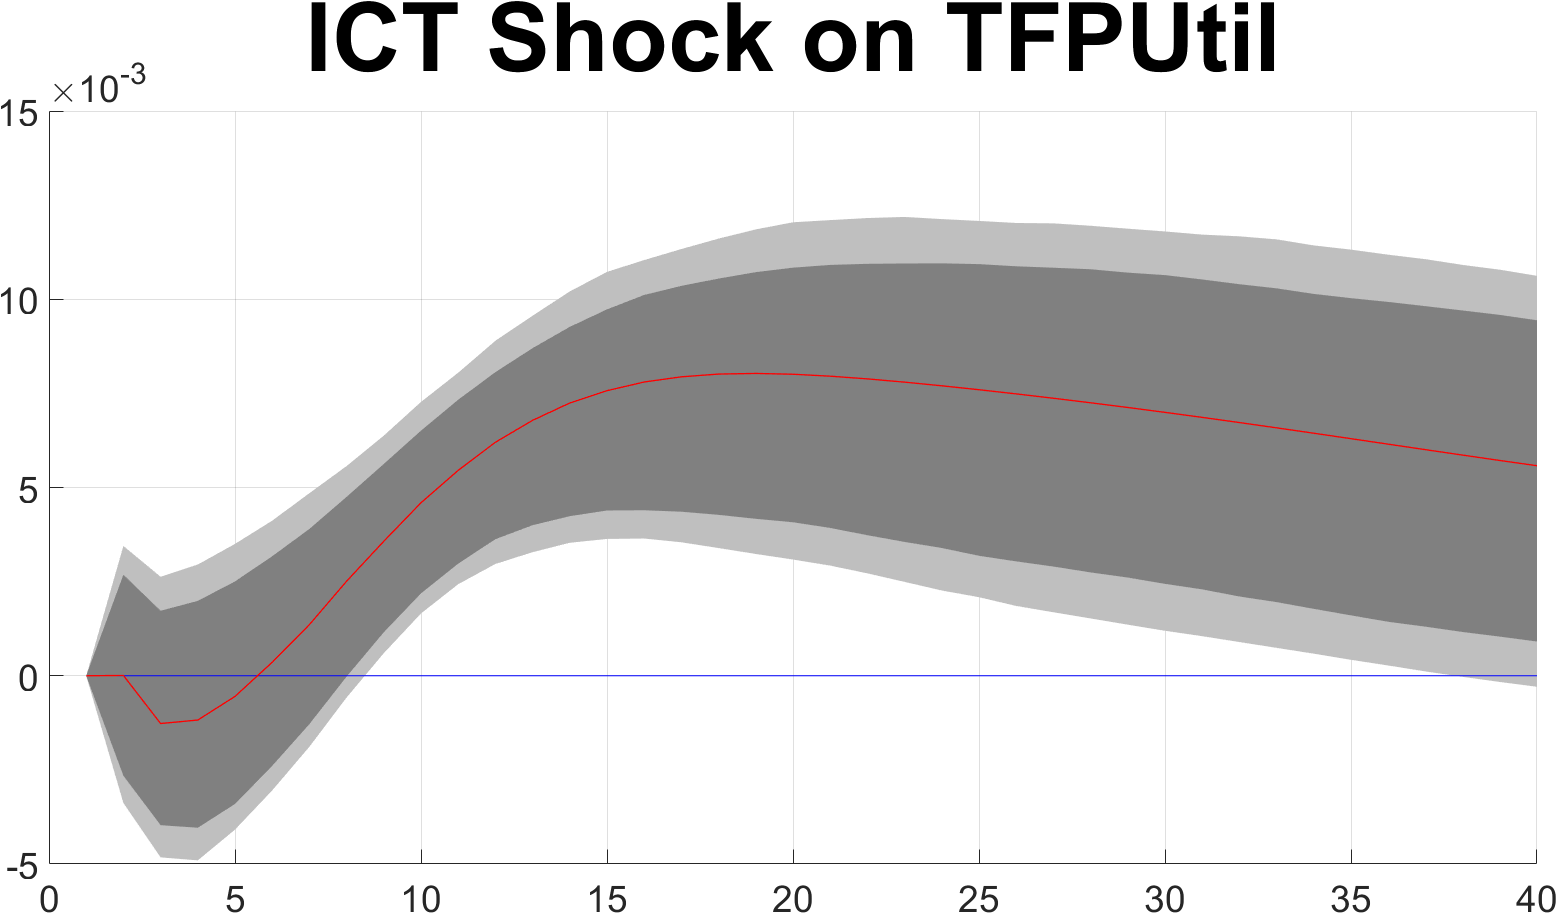
\includegraphics[scale=0.25]{fig_ICT_Shock_on_TFPUtil_empirical_fullEconomy}
		\label{fig:TFP_main}
	\end{center}
\end{figure}
}




\frame{
	\frametitle{Impulse Responses of $X_t$ to $\varepsilon_{2,t}$}


%\begin{figure}[h!]
%	\subfigure{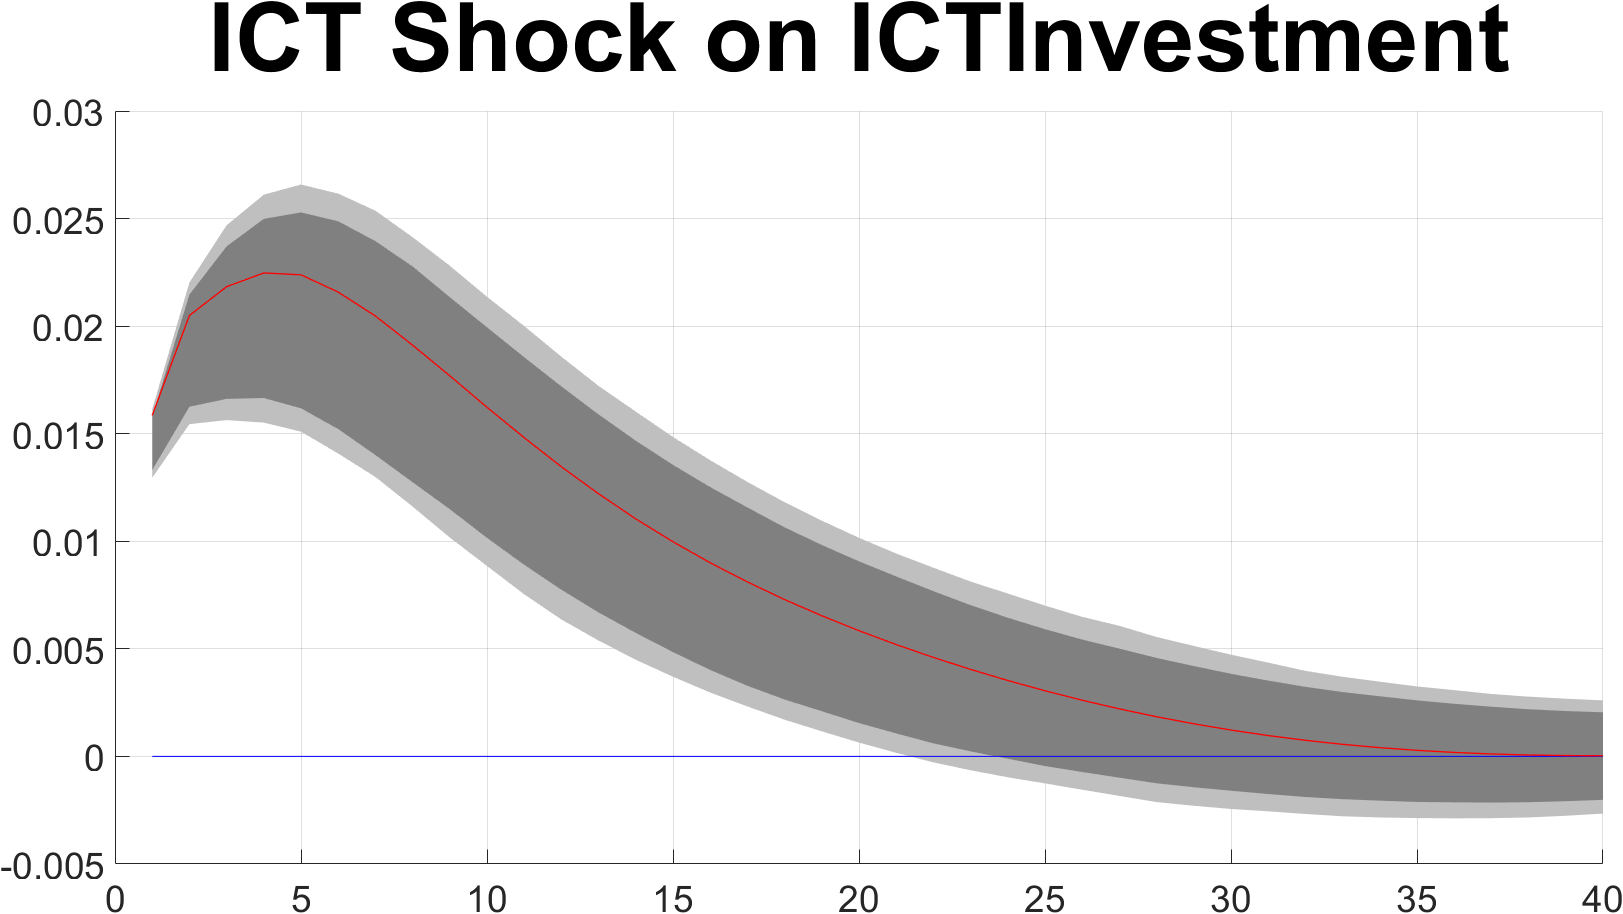
\includegraphics[width=  0.2]{fig_ICT_Shock_on_ICTInvestment_empirical_fullEconomy}} \hspace{.2in} 
%	\subfigure{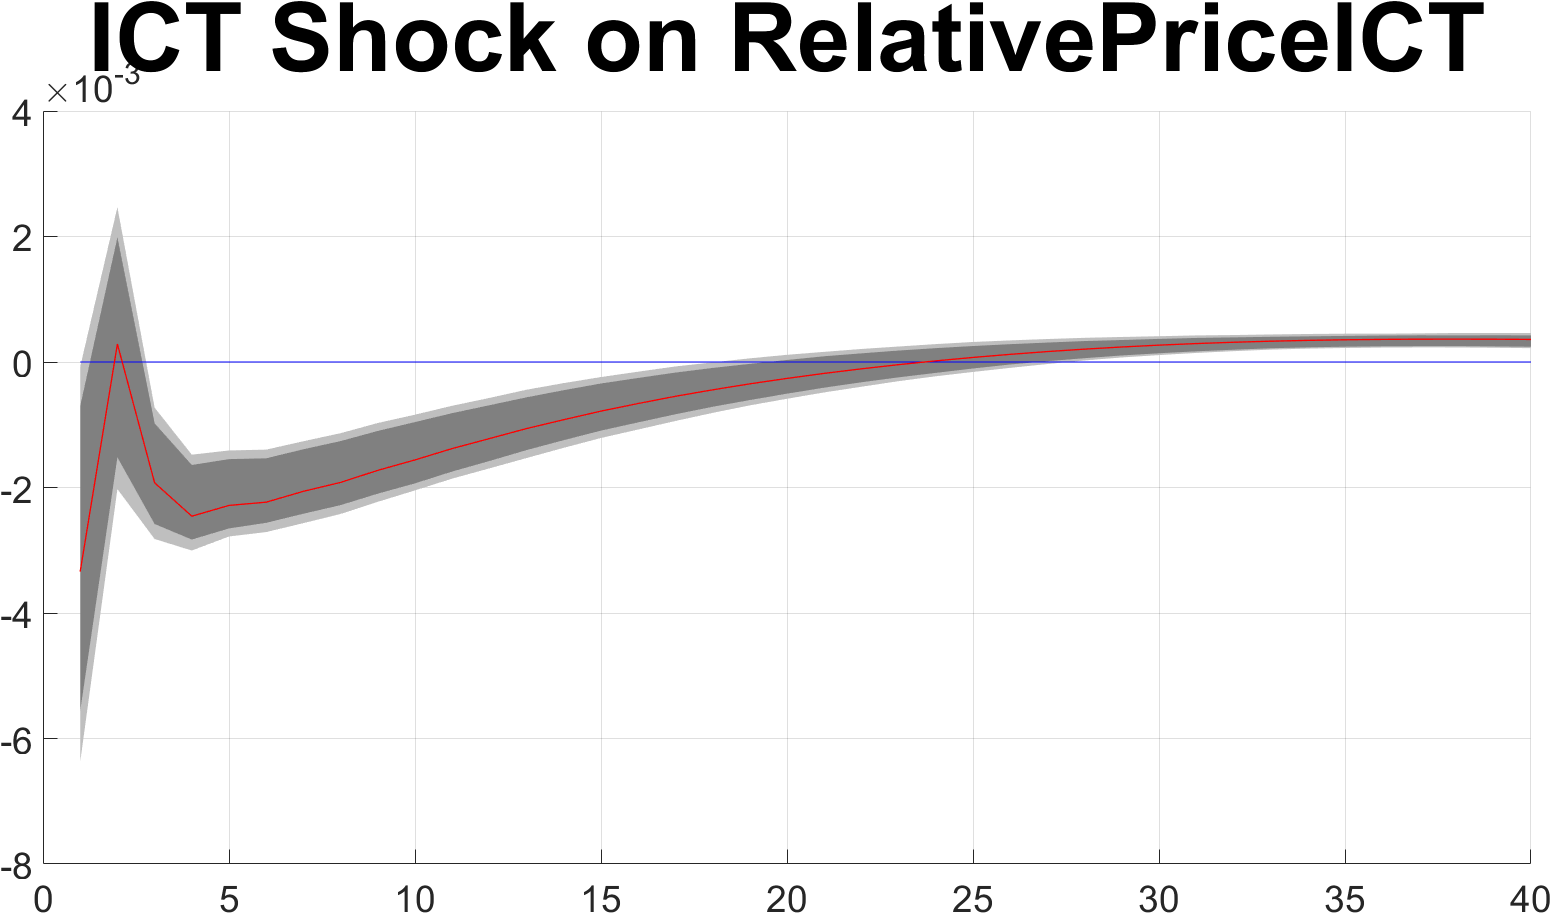
\includegraphics[width=  0.2]{fig_ICT_Shock_on_RelativePriceICT_empirical_fullEconomy}} \hspace{.2in} 
%	\subfigure{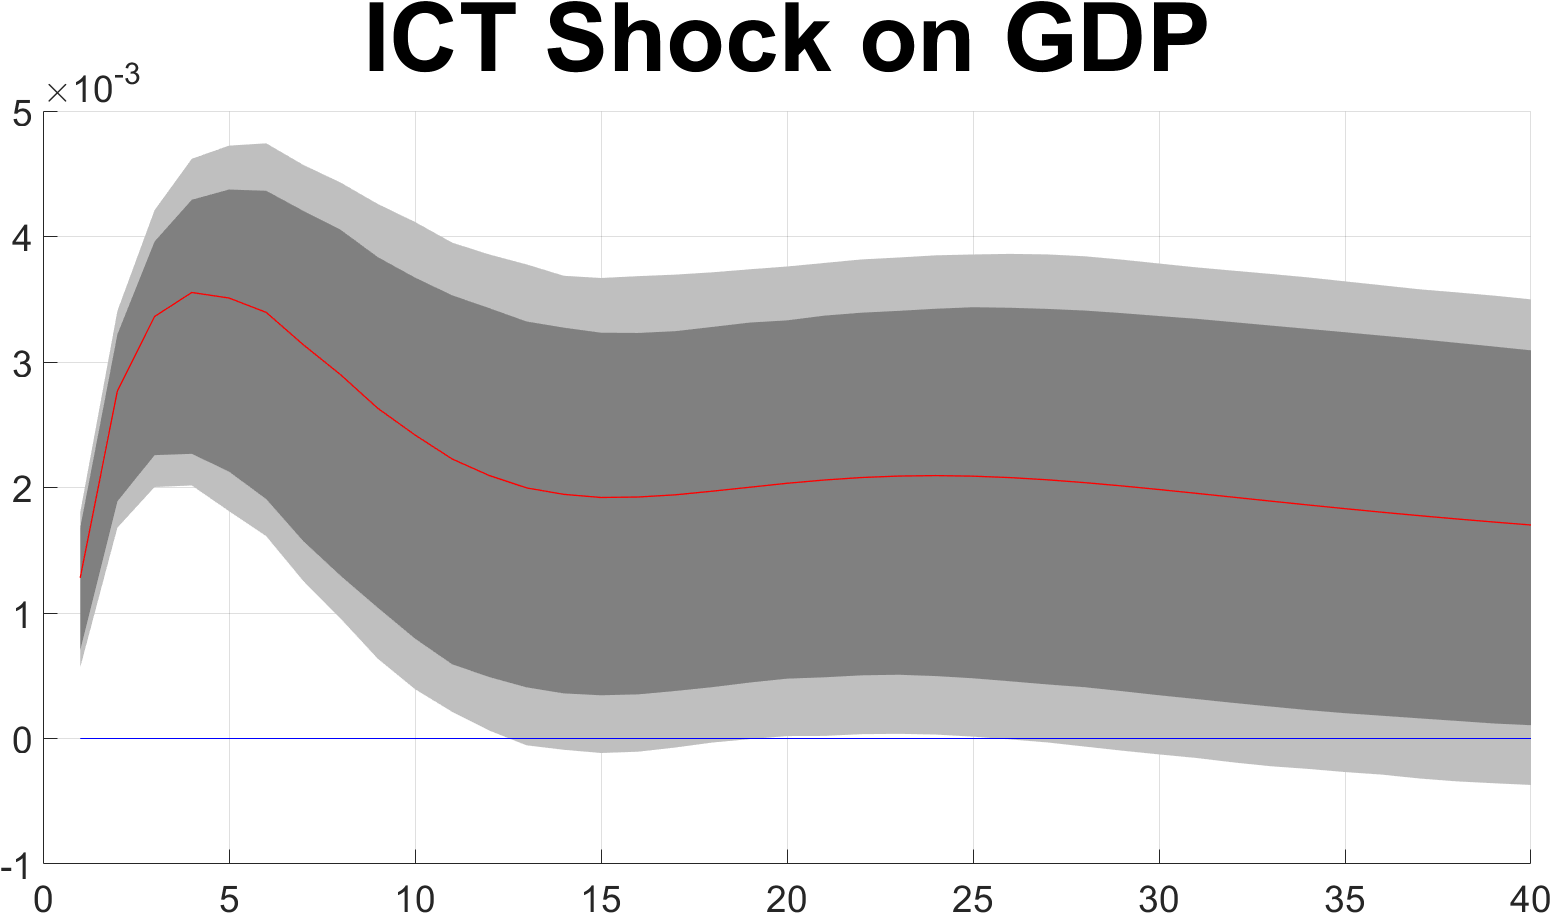
\includegraphics[width=   0.2]{fig_ICT_Shock_on_GDP_empirical_fullEconomy}} \hspace{.2in} 
%	\subfigure{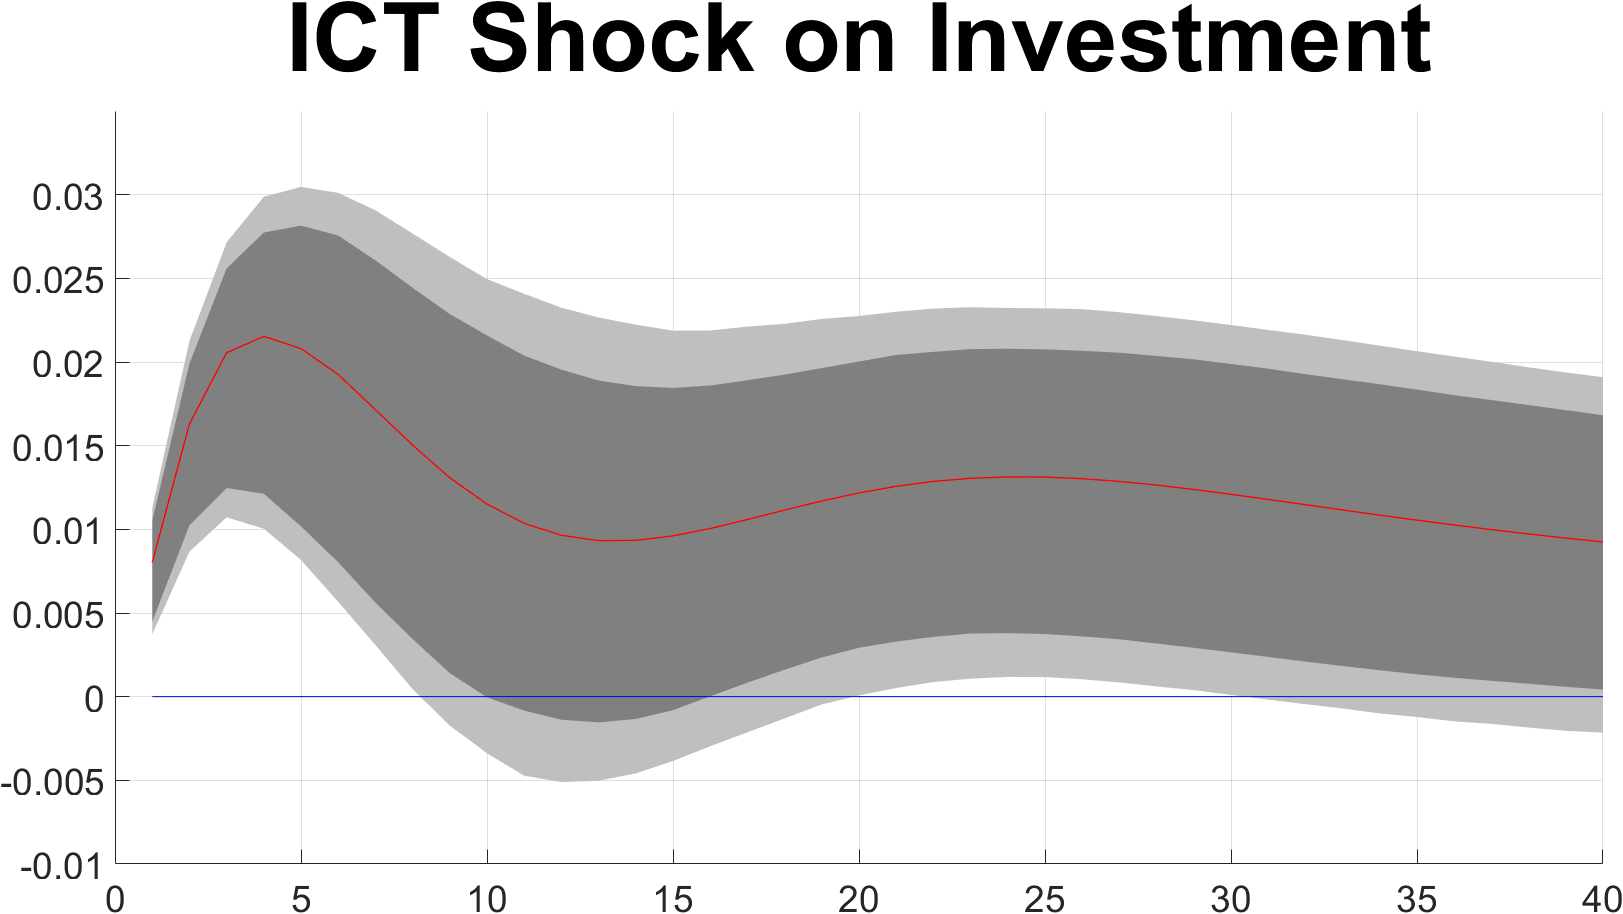
\includegraphics[width=   0.2]{fig_ICT_Shock_on_Investment_empirical_fullEconomy}} 
%\end{figure}	

\begin{figure}
	\centering
	\subfloat{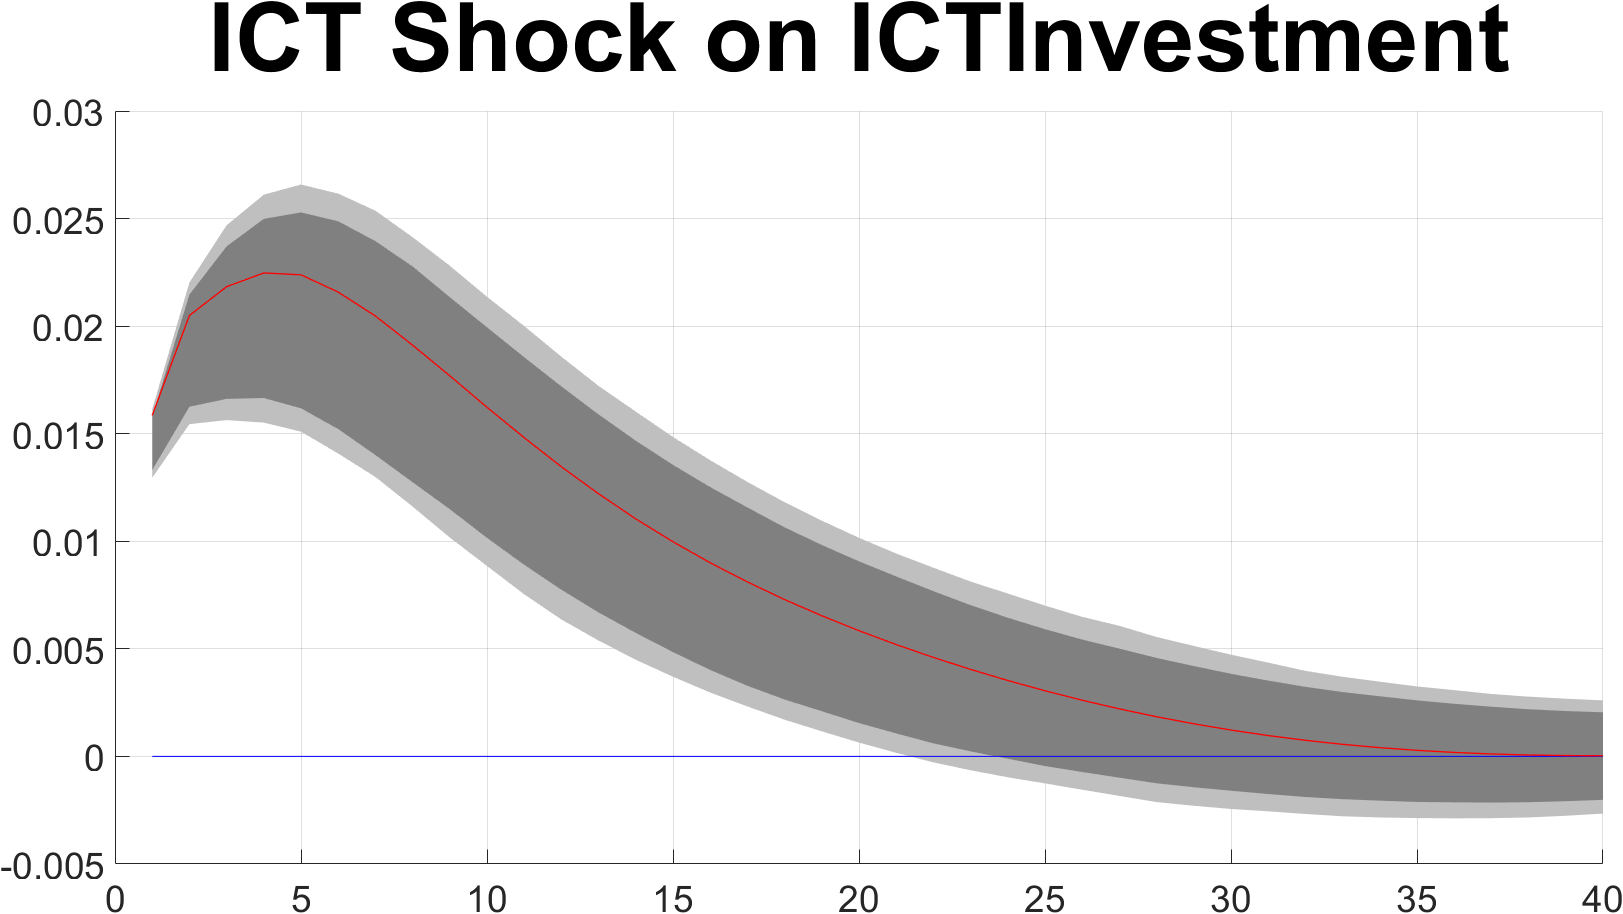
\includegraphics[height=3cm,width=3cm]{fig_ICT_Shock_on_ICTInvestment_empirical_fullEconomy}}\qquad
	\subfloat{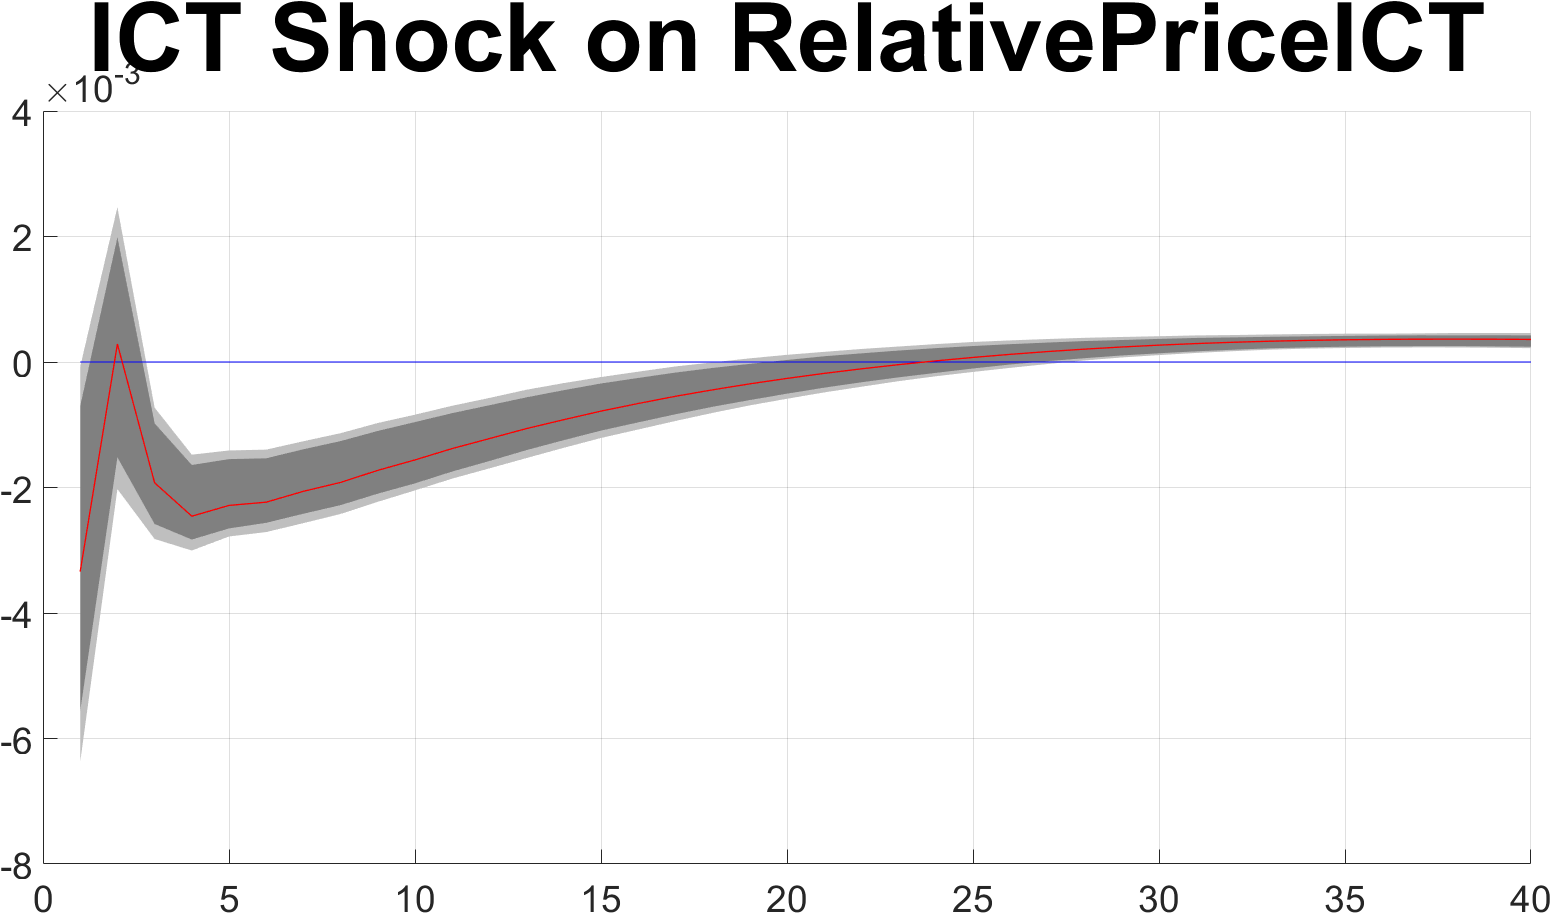
\includegraphics[height=3cm,width=3cm]{fig_ICT_Shock_on_RelativePriceICT_empirical_fullEconomy}}\qquad
	\subfloat{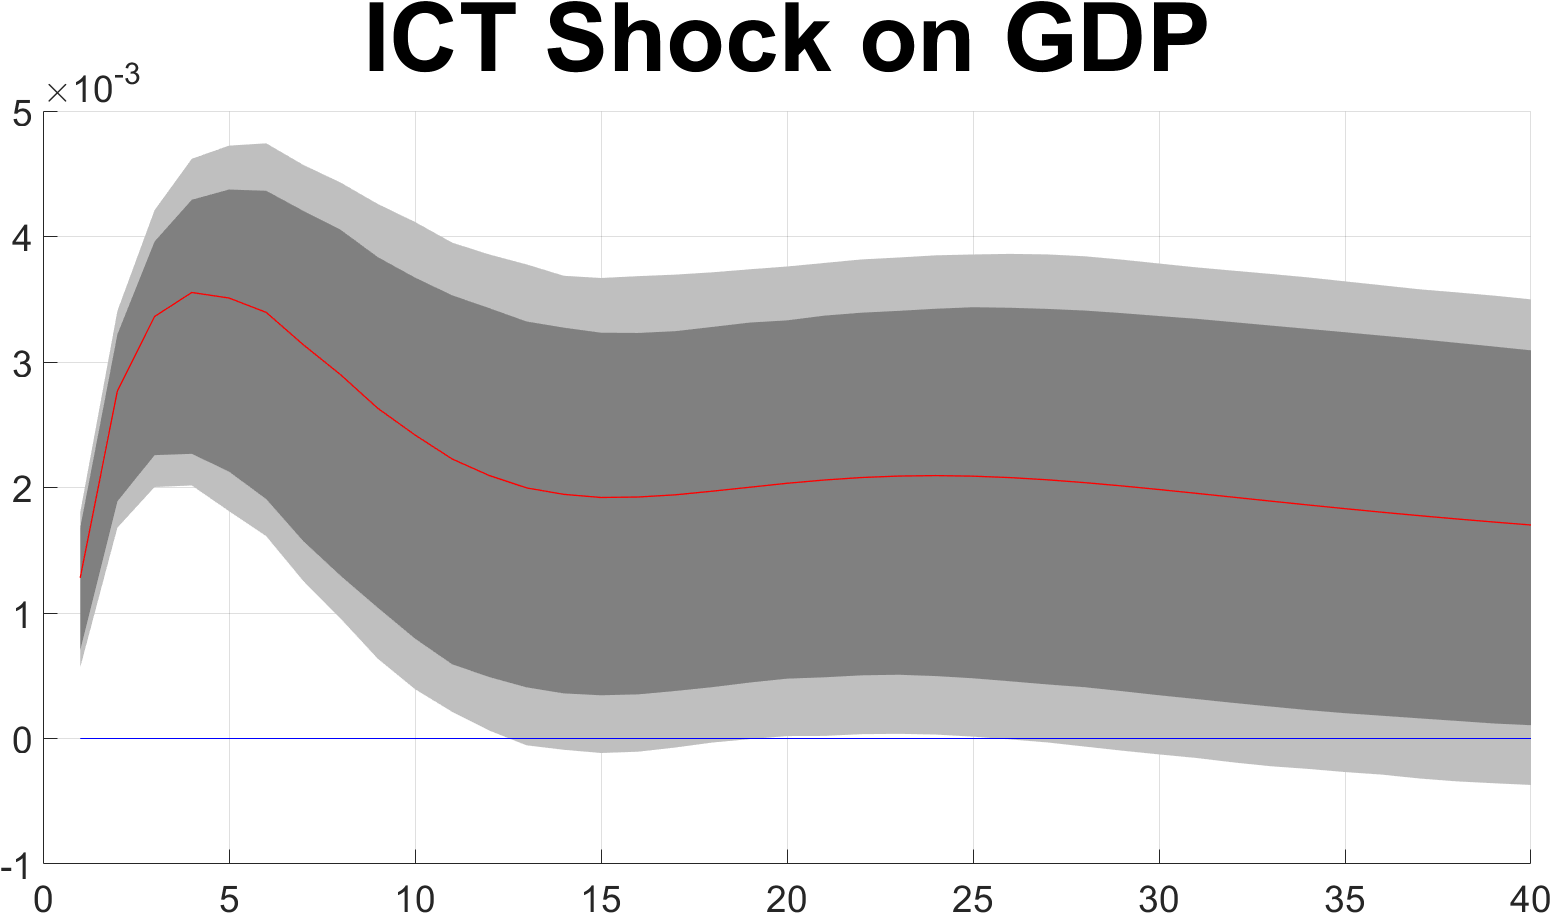
\includegraphics[height=3cm,width=3cm]{fig_ICT_Shock_on_GDP_empirical_fullEconomy}}\qquad
	
		\subfloat{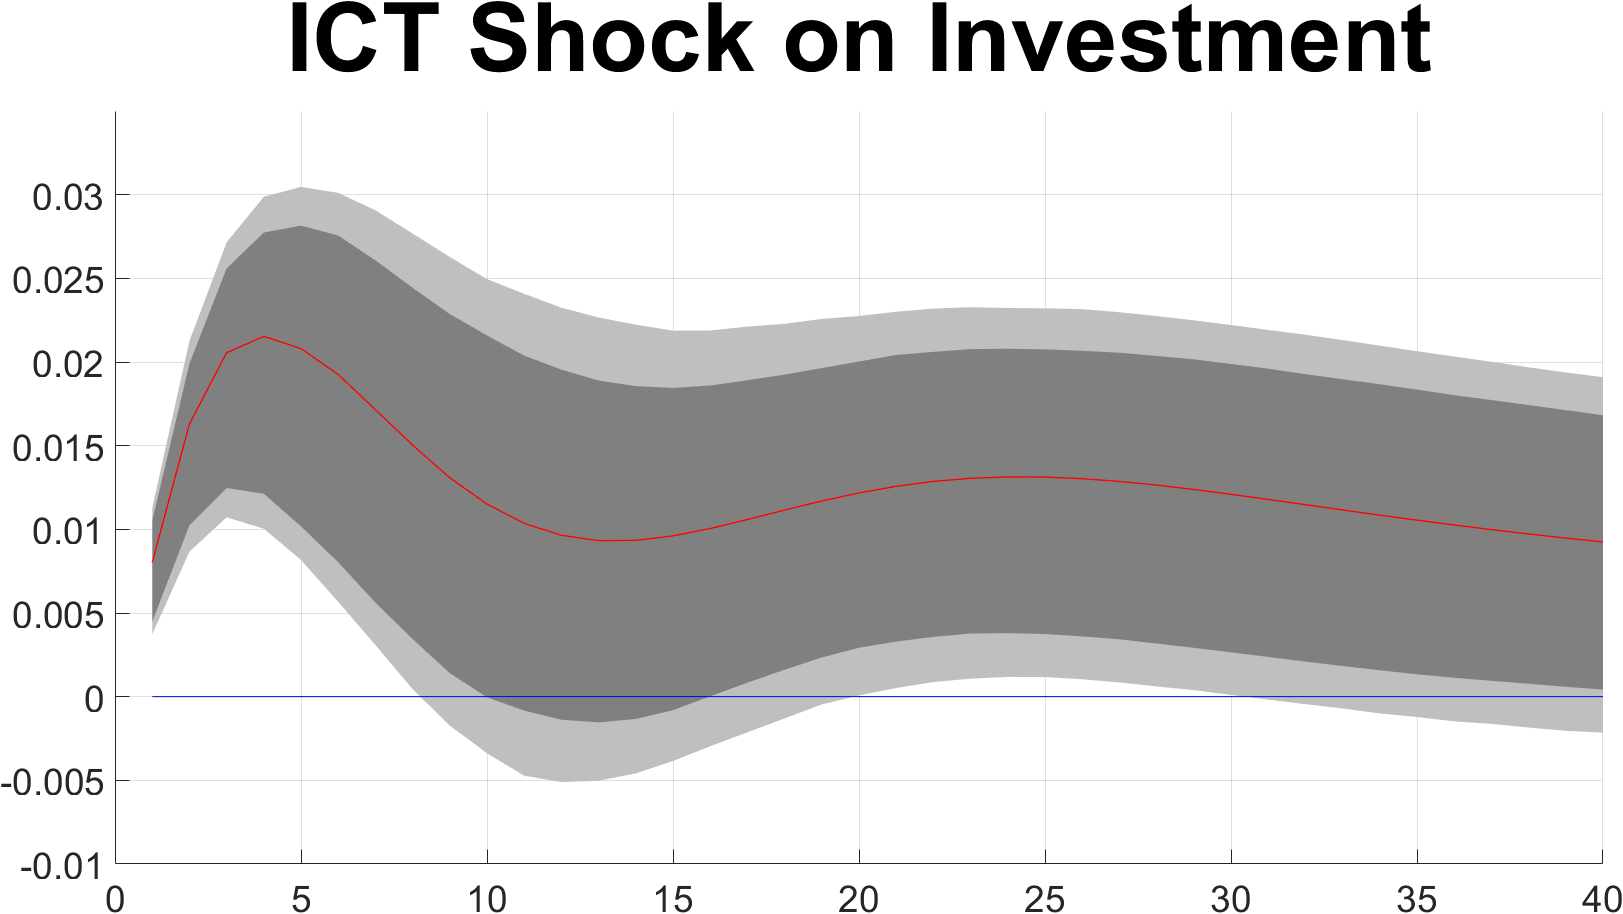
\includegraphics[height=3cm,width=3cm]{fig_ICT_Shock_on_Investment_empirical_fullEconomy}}\qquad
	\subfloat{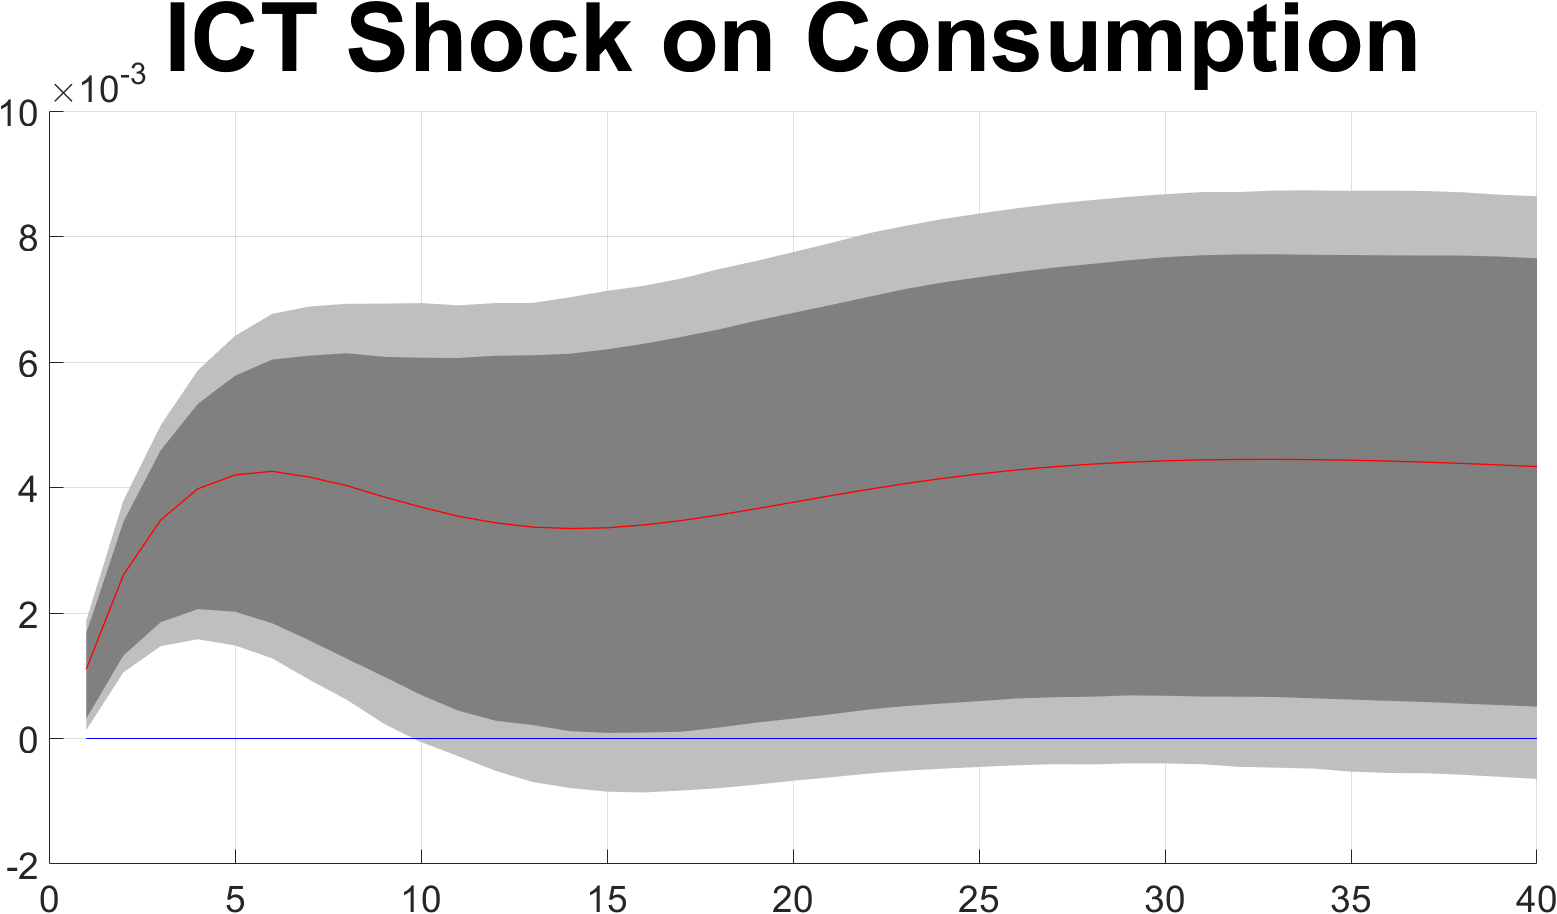
\includegraphics[height=3cm,width=3cm]{fig_ICT_Shock_on_Consumption_empirical_fullEconomy}}\qquad
	\subfloat{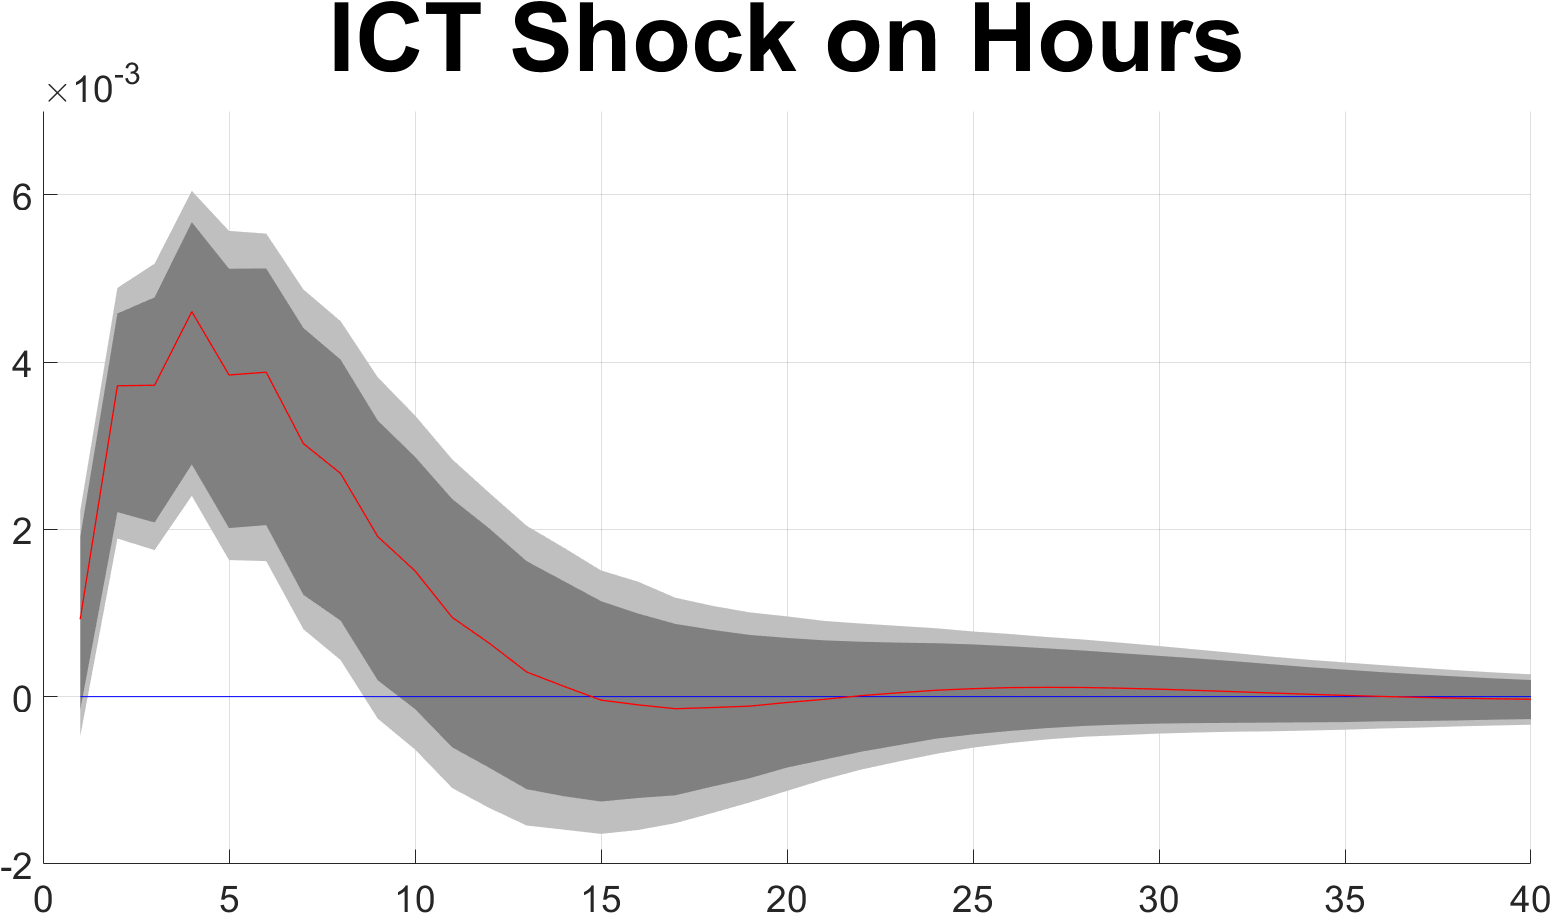
\includegraphics[height=3cm,width=3cm]{fig_ICT_Shock_on_Hours_empirical_fullEconomy}}\qquad
\end{figure}


}

	

\frame{\frametitle{Robustness Checks and Related Exercises}
	
	\begin{itemize}
		\item ICT shocks are \textbf{important driver} of business cycle fluctuations
	\begin{itemize}
		\item[-] Almost $100$\% of ICT investment on impact
		\item[-] Around $30$\% of TFP fluctuations over 10-year horizon 
		\item[-] Almost $40$\% of GDP fluctuations over BC frequencies
	\end{itemize}

\

\item \textbf{Results are robust} to
\begin{itemize}
	\item[-] Changing the available information in the system
	\begin{itemize}
	\item[$\rightarrow$] Estimated ICT shocks pass Forni-Gambetti test
	\end{itemize}
	\item[-] Not controlling for contemporaneous TFP
	\item[-] Controlling for news shocks \`a la Barsky and Sims
	\item[-] Controlling for other shocks
	\begin{itemize}
		\item[$\rightarrow$] Ramey Military News 
		\item[$\rightarrow$]  Romer-Romer Monetary Policy 
		\item[$\rightarrow$]  \dots
	\end{itemize}
\end{itemize}
\end{itemize}



}


\frame{\frametitle{Takeaway}
	
	We identify a shock specific to the ICT sector where prices and quantities move in different directions
	
	\
	
	Altough TFP does not move on impact, it start rising significantly after a couple of years
	\begin{itemize}
		\item this effect is significant and economically meaningful
	\end{itemize}

	
\begin{itemize}
	\item Supply shocks specific to the ICT sector explain a large part of medium-run TFP fluctuations
	\begin{itemize}
		\item[-] ICT prices fall relatively to CPI
	\end{itemize}
	\item Shocks which explains large part of TFP fluctuations
\end{itemize}

}
		












\end{document}